% Copyright (c) 2011 Jérémie DECOCK (http://www.jdhp.org)

\documentclass{beamer}

\usepackage[utf8]{inputenc}
\usepackage[frenchb]{babel}

\usepackage{subfigure}

%%%%%%%%%%%%%%%%%%%%%%%%%%%%%%%%%%%%%%%%%%%%%%%%%%%%%%%%%%%%%%%%%%%%%%%%%%%%%%%

% TikZ %%%%%%%%%%%%%%%%%%%%%%%%%%%%%%%%%%%%%%%%%%%%%%%%%%%%%%%%%%%%%%%%%%%%%%%%
\usepackage{bm} % bold math
\usepackage{color} % change text color
\usepackage{tikz}

\usetikzlibrary{matrix} % for block alignment
\usetikzlibrary{arrows} % for arrow heads
\usetikzlibrary{calc}   % for manimulation of coordinates
\usetikzlibrary{positioning} 
\usetikzlibrary{patterns}


%\renewcommand{\vec}[1]{\ensuremath{\boldsymbol{#1}}} % bold vectors

%%%%%%%%%%%%%%%%%%%%%%%%%%%%%%%%%%%%%%%%%%%%%%%%%%%%%%%%%%%%%%%%%%%%%%%%%%%%%%%%

% Pour désactiver temporairement les images (compile beaucoup plus vite)
%\renewcommand{\includegraphics}[2][]{\null}

% Symboles mathématiques

\def\bbbr{{\rm I\!R}} %reelle Zahlen
\newcommand{\N}{\mathbb{N}}
\newcommand{\Z}{\mathbb{Z}}
\newcommand{\Q}{\mathbb{Q}}
\newcommand{\R}{{\bbbr}{}}
\newcommand{\C}{\mathbb{C}}
\newcommand{\K}{\mathbb{K}}

\newcommand{\mb}[1]{\mathbb{#1}}
\newcommand{\mc}[1]{\mathcal{#1}}
\newcommand{\mfrac}[1]{\mathfrak{#1}}

\newcommand{\ch}    {\mathop{\mathrm{ch}}\nolimits}
\newcommand{\sh}    {\mathop{\mathrm{sh}}\nolimits}

%%% Commandes générales

\newcommand{\vs}[1]{\boldsymbol{#1}} % vector symbol (\boldsymbol, \textbf or \vec)
\newcommand{\ms}[1]{\boldsymbol{#1}} % matrix symbol (\boldsymbol, \textbf)

\newcommand{\scut}{\text{sc}}        % shortcut symbol

\newcommand{\ostate}{\vs{\chi}}        % state in operational space
\newcommand{\dostate}{\vs{\dot{\chi}}} % derivative of the state in operational space
\newcommand{\x}{\vs{x}}                % cartesian position vector
\newcommand{\xx}{x_1}                  % x
\newcommand{\xy}{x_2}                  % y
\newcommand{\dx}{\vs{\dot{x}}}
\newcommand{\dxx}{\dot{x}_1}
\newcommand{\dxy}{\dot{x}_2}
\newcommand{\ddx}{\vs{\ddot{x}}}
\newcommand{\ddxx}{\ddot{x}_1}
\newcommand{\ddxy}{\ddot{x}_2}

\newcommand{\jstate}{\vs{\xi}}         % state in joint space
\newcommand{\djstate}{\vs{\dot{\xi}}}  % derivative of the state in joint space
\newcommand{\q}{\vs{q}}                % joint vector
\newcommand{\qs}{q_1}                  % shoulder angle
\newcommand{\qe}{q_2}                  % elbow angle
\newcommand{\cosqs}{\cos(\qs)}
\newcommand{\cosqe}{\cos(\qe)}
\newcommand{\cosqsqe}{\cos(\qs + \qe)}
\newcommand{\sinqs}{\sin(\qs)}
\newcommand{\sinqe}{\sin(\qe)}
\newcommand{\sinqsqe}{\sin(\qs + \qe)}
\newcommand{\dq}{\vs{\dot{q}}}
\newcommand{\dqs}{\dot{q}_1}
\newcommand{\dqe}{\dot{q}_2}
\newcommand{\ddq}{\vs{\ddot{q}}}
\newcommand{\ddqs}{\ddot{q}_1}
\newcommand{\ddqe}{\ddot{q}_2}

\newcommand{\mstate}{\mathcal{U}}         % state in joint space

\newcommand{\rewardfactor}{\rho}       % reward factor
\newcommand{\costfactor}{\epsilon}     % cost factor
\newcommand{\discountfactor}{\gamma}   % discount factor
\newcommand{\discountfunction}{\Gamma}   % discount factor

\newcommand{\costfuntion}{\mathcal{C}}
\newcommand{\costfuntionhat}{\hat{\mathcal{C}}}

\newcommand{\fk}{\vs{\mathcal{FK}}}
\newcommand{\processfuntion}{\vs{\mathcal{PF}}}

\newcommand{\octrl}{\vs{\phi}}  % control in operational space
\newcommand{\jctrl}{\vs{u}}  % control in joint space

\newcommand{\dcm}{a}            % distance séparant le centre ... au centre de masse de ...
\newcommand{\dcmu}{a_1}         % distance séparant le centre de l'épaule au centre de masse du bras
\newcommand{\dcmf}{a_2}         % distance séparant le centre du coude au centre de masse de l'avant bras

\newcommand{\vt}{\vs{\tau}}          % torque vector
\newcommand{\ts}{\tau_1}             % shoulder torque
\newcommand{\te}{\tau_2}             % elbow torque

\newcommand{\len}{l}                 % arm length
\newcommand{\lu}{l_1}                % upper arm length
\newcommand{\lf}{l_2}                % forearm length

\newcommand{\m}{m}                   % mass
\newcommand{\msu}{m_1}               % forearm mass
\newcommand{\mf}{m_2}                % forearm mass

\newcommand{\si}{\iota}             % moment of inertia scalar
\newcommand{\is}{\iota_1}           % shoulder moment of inertia
\newcommand{\ie}{\iota_2}           % elbow moment of inertia

\newcommand{\invM}[1]{M^{-1}_{#1}}  % inverse de la matrice d'inertie
\newcommand{\detM}{\det(\ms{M})}

\newcommand{\deriv}[2]{\frac{d {#1}}{d {#2}}}  % derivative
\newcommand{\pd}[2]{\frac{\partial {#1}}{\partial {#2}}}  % partial derivative

\newcommand{\jacobian}{\ms{J}}             % jacobienne (matrice)
\newcommand{\djacobian}{\ms{\dot{J}}}
\newcommand{\ddjacobian}{\ms{\ddot{J}}}

\newcommand{\motornoise}{w}
\newcommand{\vmotornoise}{\vs{w}}

\newcommand{\perceptionnoise}{\nu}
\newcommand{\vperceptionnoise}{\vs{\nu}}

\newcommand{\then}{\Rightarrow}
\newcommand{\alias}{\triangleq}
%\newcommand{\argmin}{\operatornamewithlimits{argmin}}

%\newcommand{\reels}{\mathbb{R}}
%\newcommand{\equiv}{\Leftrightarrow}
%\renewcommand{\det}[1]{\det({#1})}
%\numberwithin{equation}{subsection}
%\setlength\arraycolsep{5.4pt}
%\setlength\arrayrulewidth{15.4pt}
%\renewcommand\arraystretch{1.5}

\newenvironment{jmatrix}{\renewcommand\arraystretch{1.5} \begin{pmatrix}}{\end{pmatrix}}

\newcommand{\todo}[1][\dots]{\textbf{[TODO : #1]}}  % todo mark

\newcommand{\HRule}{\rule{\linewidth}{0.5mm}}

\newcommand{\dontforget}[1]{\textcolor{red}{#1}}
\newcommand{\qopsx}{\text{QOPS}_\phi}
\newcommand{\qopslqp}{\text{QOPS}_\phi\text{+LQP}}



%%%%%%%%%%%%%%%%%%%%%%%%%%%%%%%%%%%%%%%%%%%%%%%%%%%%%%%%%%%%%%%%%%%%%%%%%%%%%%%

\usetheme[compress]{Dresden}

\title{Optimisation du contrôle moteur}
\subtitle{Vers un modèle structuré}

% \author[⟨short author names⟩]{⟨author names⟩}
% The names should be separated using the command \and.
\author[Decock]{Jérémie~\bsc{Decock}\\\medskip{\small {\em Superviseur~:} Olivier~\bsc{Sigaud}}}

\institute{UPMC ~~~ ISIR}
\date{07 septembre 2011}

% \subject{⟨text⟩}
% Enters the ⟨text⟩ as the subject text in the pdf document info.
% It currently has no other effect.
\subject{contrôle moteur}

% \keywords{⟨text⟩}
% Enters the ⟨text⟩ as keywords in the pdf document info.
% It currently has no other effect. 
\keywords{contrôle moteur, robotique}

\AtBeginSection[] {
    \begin{frame}
    \begin{center}
        {\LARGE \insertsectionhead}
    \end{center}
    \end{frame}
}

%\AtBeginSection[] {
%    %\begin{frame}<beamer>{Plan}
%    \begin{frame}<beamer>
%        \tableofcontents[currentsection]
%    \end{frame}
%}

%\AtBeginSection[] {
%    %\begin{frame}<beamer>{Plan}
%    \begin{frame}<beamer>
%        \tableofcontents[currentsection,currentsubsection]
%    \end{frame}
%}
%
%\AtBeginSubsection[] {
%    %\begin{frame}<beamer>{Plan}
%    \begin{frame}<beamer>
%        \tableofcontents[currentsection,currentsubsection]
%    \end{frame}
%}

%%%%%%%%%%%%%%%%%%%%%%%%%%%%%%%%%%%%%%%%%%%%%%%%%%%%%%%%%%%%%%%%%%%%%%%%%%%%%%%

\begin{document}

% Défini le logo
\logo{\includegraphics[height=0.5cm]{fig/logo_upmc}}

\begin{frame}
    \titlepage
\end{frame}

% Redéfini le logo : pour tous les slides suivants
% logo est remplacé par le numéro de page
\setbeamercolor*{logo}{fg=black}
\logo{\insertframenumber}
%\logo{\insertframenumber/\inserttotalframenumber}

%%%%%%%%%%%%%%%%%%%%%%%%%%%%%%%%%%%%%%%%%%%%%%%%%%%%%%%%%%%%%%%%%%%%%%%%%%%%%%%

\section*{Introduction}

\subsection*{Introduction}

\begin{frame}{Le contrôle moteur}
    \begin{block}{But}
        Amener un {\em système mécanique} d'un {\em état} initial à un état désiré
        \begin{center}
            \includegraphics[width=.40\linewidth]{fig/path}
        \end{center}
    \end{block}
\end{frame}

\begin{frame}{La boucle de contrôle}
    \begin{center}
        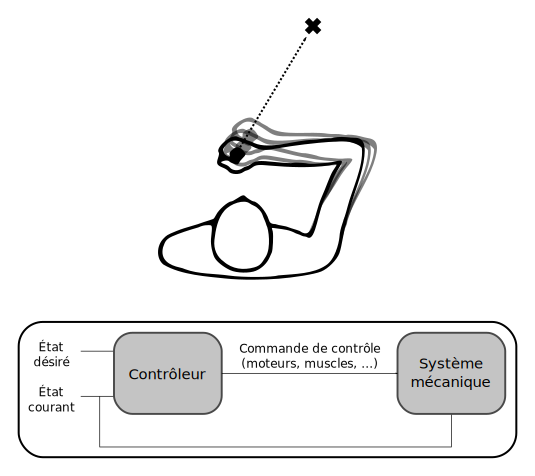
\includegraphics[width=.70\linewidth]{fig/ctrl2}
    \end{center}
\end{frame}

\begin{frame}{Nos objectifs}
    \begin{columns}
        \begin{column}{0.50\textwidth}
            \begin{itemize}
                \item Faire du contrôle moteur sur un système complexe 
                \item Générer des mouvements réalistes et efficaces en reproduisant les propriétés connues du contrôle moteur humain
                %\item Faire un contrôleur pouvant être appris avec les techniques actuelles d'IA
            \end{itemize}
        \end{column}
        \begin{column}{0.50\textwidth}
            \begin{center}
                \includegraphics[width=.95\linewidth]{fig/icub_light}
            \end{center}
        \end{column}
    \end{columns}
\end{frame}

\subsection*{Problématique}

\begin{frame}{Problèmes}
    \begin{small}
        Les techniques actuelles ne permettent pas de remplir ces 2 conditions à la fois~:
        ~\\
        \begin{columns}
            \begin{column}{0.70\textwidth}
                \begin{block}{Robotique}
                    Systèmes complexes mais mouvement pas \og{}réaliste\fg{} et peu \og{}efficace\fg{} %pas \og{}human like\fg{} $[$RMRC, Toussaint, ...$]$
                \end{block}
                \begin{block}{Contrôle moteur}
                    Systèmes simples seulement %$[$Rigoux et Guigon, Todorov, ...$]$
                \end{block}
                %\begin{block}{IA - Apprentissage}
                %    Systèmes simples seulement (\og{}malédiction de la dimensionalité\fg{})
                %    %\og{}Malédiction de la dimensionalité\fg{} en apprentissage
                %\end{block}
            \end{column}
            \begin{column}{0.30\textwidth}
                \begin{center}
                    \includegraphics[width=.95\linewidth]{fig/asimo}
                \end{center}
            \end{column}
        \end{columns}
    \end{small}
\end{frame}

%\subsection{Problématique}
%
%%%%%%%%%%%%%%%%%%%%%%%%%%%%%%%%%%%%%%%%
%
%\begin{frame}{Introduction}
%    \begin{figure}
%        \centering
%        \subfigure[Corps humain]{\includegraphics[width=.50\linewidth]{fig/arm4}}~~~
%        \subfigure[Système mécanique poly-articulé]{\includegraphics[width=.50\linewidth]{fig/arm1}}
%    \end{figure}
%\end{frame}
%
%\begin{frame}{Introduction}
%    \begin{small}
%        \begin{itemize}
%            \item Système mécanique défini par un état (vitesse position)
%            \item L'état peut être décrit dans plusieurs espaces
%        \end{itemize}
%    \end{small}
%    \begin{figure}[ht]
%        \centering
%        \input{tikz/tikz_slides_arm_space.tex}
%    \end{figure}
%    \begin{small}
%    Notations : état  $\jstate = \begin{pmatrix} \dq & \q \end{pmatrix}^T$ et 
%    $\ostate = \begin{pmatrix} \dx & \x \end{pmatrix}^T$
%    \end{small}
%\end{frame}
%
%%\begin{frame}{Problématique}
%%    Redondant dans l'espace de la tâche
%%    \begin{center}
%%        \includegraphics[width=.40\linewidth]{fig/arm2}
%%    \end{center}
%%\end{frame}
%
%\begin{frame}{Problématique}
%    \begin{block}{Une question clé}
%        Pourquoi réalise-t-on tel mouvement plutôt qu'un autre~? $[$Bernstein~67$]$
%    \end{block}
%    \begin{center}
%        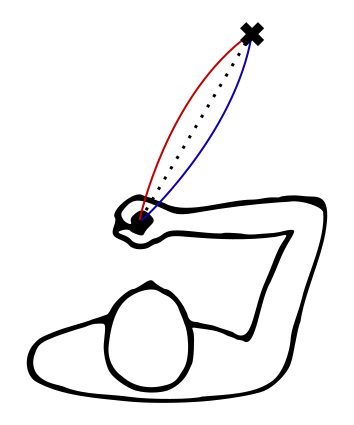
\includegraphics[width=.40\linewidth]{fig/paths}
%    \end{center}
%\end{frame}
%
%%%%%%%%%%%%%%%%%%%%%%%%%%%%%%%%%%%%%%%%
%
%\begin{frame}{Un début de réponse\dots}
%    \begin{block}{Un processus d'optimisation~?}
%        \begin{itemize}
%            \item Pourquoi deux tâches identiques produisent des mouvements différents ?
%            \item Peut-on quantifier ces variations ?
%        \end{itemize}
%    \end{block}
%    Plusieurs propriétés du contrôle moteur ont été identifiées
%    \begin{block}{Principes clés~:}
%        \begin{itemize}
%            \item Minimisation de la variance au point final
%            \item Principe d'intervention minimum
%        \end{itemize}
%    \end{block}
%\end{frame}
%
%%%%%%%%%%%%%%%%%%%%%%%%%%%%%%%%%%%%%%%%
%
%\begin{frame}{Des pistes d'améliorations}
%    Contrôleur de $[$Rigoux et Guigon 11$]$
%    \begin{itemize}
%        \item Reproduit les propriétés du contrôle moteur
%        \item Mais\dots optimise les actions musculaires $\Rightarrow$ trop lent
%    \end{itemize}
%    Regarder le problème sous un autre angle~:
%    \begin{itemize}
%        \item Cinématique
%        \item Dynamique
%        \item Actionnement
%    \end{itemize}
%    Peut-on optimiser sur un plus petit espace ?
%\end{frame}



\begin{frame}{Plan}
    \tableofcontents
\end{frame}

\section{Présentation de l'existant}

\subsection{Le contrôleur QOPS}

\begin{frame}{Réalisme et efficacité}
    On veut des mouvements réalistes et efficaces
    \begin{itemize}
        \item Optimiser~: choisir le \og{}meilleur\fg{} mouvement parmi tous ceux qui permettent de résoudre la tâche
        %\item Celui qui minimise son coût énergétique et maximise sa vitesse
    \end{itemize}
    \begin{center}
        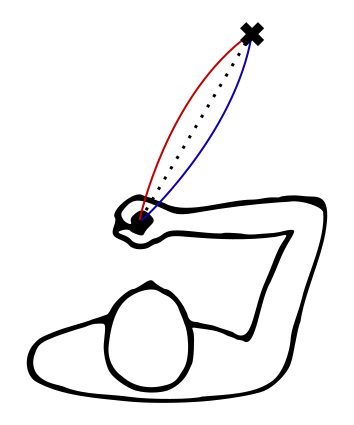
\includegraphics[width=.35\linewidth]{fig/paths}
    \end{center}
\end{frame}

\begin{frame}{Le contrôleur QOPS $[$Rigoux et Guigon 11$]$}
    QOPS présente de bonnes propriétés et on aimerait l'utiliser~:
    \begin{itemize}
        \item Efficace~: trouve le mouvement optimal même en présence de bruit
        \begin{itemize}
            \item Minimise les dépenses énergétiques
            \item Maximise la vitesse
        \end{itemize}
        \item Réaliste~: reproduit les propriétés connues du contrôle moteur humain
    \end{itemize}
%    ~\\
%    Mais~:
%    \begin{itemize}
%        \item il coûte cher en calculs
%        \item on ne peut pas l'utiliser que sur des systèmes simples (bras avec deux articulations seulement)
%    \end{itemize}
\end{frame}

\begin{frame}{Le contrôleur QOPS}
    QOPS permet de contrôler des systèmes mécaniques actionnés par des muscles
    ~\\
    \begin{block}{Pourquoi s'intéresser à un modèle avec muscles~?}
        \begin{itemize}
            \item La robotique s'oriente vers ce type d'actionneurs
            \item Permettent d'avoir des propriétés intéressantes~: réguler la raideur
            \item À terme, profiter de l'énergie cinétique du système avec des muscles élastiques
        \end{itemize}
    \end{block}
\end{frame}

\begin{frame}{Le contrôleur QOPS}
    %Des calculs coûteux~:
    \begin{itemize}
        %\item Utilise une méthode de {\em calcul variationnel} pour trouver le meilleur mouvement pour aller de l'état courant $\jstate$ à l'état désiré $\jstate^*$
        \item Utilise une méthode de {\em calcul variationnel} pour trouver la meilleur commande $\jctrl^*$ qui permet de s'approcher de l'état désiré $\jstate^*$ connaissant l'état courant $\jstate$
        \item État = position et vitesse angulaire des articulations ($\jstate$)
        \item Commande = activations musculaires ($\jctrl$)
    \end{itemize}
    ~\\
    \begin{figure}
        \centering
       % \subfigure{\includegraphics[width=.15\linewidth]{fig/esp_ar}}~~
        \begin{tikzpicture}[scale=1, auto, >=stealth']
    \small

    \tikzstyle{blk} = [rectangle, rounded corners, draw=black, very thick, text width=8cm, minimum height=2cm, text centered]
    \tikzstyle{lab} = [rectangle]
    \tikzstyle{line} = [thick]
    \tikzstyle{connector} = [->,thick]

    %\node [blk] (qopsbox) {$$\jctrl^* = \arg\min_{\discountfactor,t_f} -\rewardfactor~e^{\frac{-t_f.\Delta_t}{\discountfactor}}  + \costfactor~\sum^{t_f}_{t=0} e^{\frac{-t.\Delta_t}{\discountfactor}} \jctrl^2~\Delta_t$$};
    \node [blk] (qopsbox) {$$\jctrl^* = \arg\min_{\jctrl,t_f} \underbrace{\costfactor~\sum^{t_f}_{t=0} \discountfunction(t_f) \jctrl^2~\Delta_t}_\text{coût énergétique} - \underbrace{\rewardfactor~\discountfunction(t_f)}_\text{récompense}$$};
    \node [lab, below of=qopsbox, node distance=1.5cm] (lableqops) {QOPS};

    % Now link the nodes %%%%%%%%%%%%%%%%%%%%%%%%%%%%%%%%%%%%%%%%%%%%%%%%%%%%%%%%%%%%%%%%
    \draw [line]      ($(qopsbox.west) + (0mm,  5mm)$) -- ($(qopsbox.west) + (-5mm,  5mm)$) node[left] {$\jstate$};
    \draw [line]      ($(qopsbox.west) + (0mm, -5mm)$) -- ($(qopsbox.west) + (-5mm, -5mm)$) node[left] {$\jstate^*$};
    \draw [connector] ($(qopsbox.east) + (0mm,  0mm)$) -- ($(qopsbox.east) + ( 5mm,  0mm)$) node[right] {$\jctrl^*$};

\end{tikzpicture}


       % \subfigure{
\includegraphics[width=.15\linewidth]{fig/ctrl_u}}
    \end{figure}
    %Compromis vitesse/effort
\end{frame}

\begin{frame}{Le contrôleur QOPS}
    \begin{itemize}
        \item Contrôleur déterministe
        %\item Temps discret
        \item Environnement bruité
        \item Mouvement recalculé à chaque pas de temps
    \end{itemize}
    \begin{figure}
        \centering
        \begin{tikzpicture}[scale=1, auto, >=stealth']
    \small

    % TikZ styles for drawing %%%%%%%%%%%%%%%%%%%%%%%%%%%%%%%%%%%%%%%%%%%%%%%%%%%%%%
    \tikzstyle{block} = [draw,rectangle,thick,minimum height=2em,minimum width=2em]
    \tikzstyle{rounded} = [draw,rectangle,rounded corners=2mm,thick,minimum height=2em,minimum width=2em]
    \tikzstyle{sum} = [draw,circle,inner sep=0mm,minimum size=2mm]
    \tikzstyle{connector} = [->,thick]
    \tikzstyle{line} = [thick]
    \tikzstyle{branch} = [circle,inner sep=0pt,minimum size=1mm,fill=black,draw=black]

    % Node placement with matrix library (3x5 array) %%%%%%%%%%%%%%%%%%%%%%%%%%%%%%%%%%%%
    \matrix[ampersand replacement=\&, row sep=0.2cm, column sep=0.5cm] {

      % row 1
      \node[branch, yshift=-2mm] (b2) {}; \&
      \node[block] (control) {Contrôleur}; \&
      \node[rounded] (noise) {Bruit}; \&
      \node[branch] (b3) {}; \&
      \node[block] (model) {Système mécanique (bras)};
      \\

      % row 2
      \&
      \node[sum] (kalman) {K}; \&
      \&
      \&
      \\

      % row 3
      \&
      \&
      \node[rounded] (delta) {Délai}; \&
      \&
      \node[branch] (b4) {};
      \\
    };

     % Now link the nodes %%%%%%%%%%%%%%%%%%%%%%%%%%%%%%%%%%%%%%%%%%%%%%%%%%%%%%%%%%%%%%%%
     \draw [line]      ($(control.west) + (-1cm, 2mm)$) -- ($(control.west) + (-1cm, 2mm)$) node[left] {$\jstate^*$};
     \draw [line]      (b2) -- ($(control.west) + (-1cm, -2mm)$) node[left] {$\jstate_0$};
     \draw [connector] ($(control.west) + (-1cm, 2mm)$) -- ($(control.west) + (0, 2mm)$);
     \draw [connector] (b2) -- ($(control.west) + (0, -2mm)$);
     \draw [connector] (control) -- node {$\jctrl$} (noise);
     \draw [line]      (noise) -- node {$\tilde{\jctrl}$} (b3);
     \draw [connector] (b3) -- (model);
     \draw [connector] (b3) |- (kalman);
     \draw [line]      (model) -- node {$\jstate_{t+1}$} (b4);
%     \draw [connector] (b4) -- ++(2.5cm,0) -- ++(0,3cm) -- ++(-2.5cm,0) -- node {$\jstate_t$} (model.north);
     \draw [connector] (b4) -- (delta);
     \draw [connector] (delta) -| (kalman);
     \draw [line]      (kalman) -| node[pos=0.20] {$\tilde{\jstate}$} (b2);

\end{tikzpicture}

    \end{figure}
\end{frame}

\subsection{Les limites de QOPS}

\begin{frame}{Les limites de QOPS}
    QOPS génère des mouvements efficaces et réalistes mais\dots
    \begin{itemize}
        \item On ne peut pas l'utiliser sur autre chose que des systèmes simples (bras avec deux articulations)
        \item Les méthodes de calcul variationnel coûtent chères en calculs
    \end{itemize}
\end{frame}

\begin{frame}{Les causes de ces limites~?}
    \begin{small}
        Le temps nécessaire pour trouver le meilleur mouvement augmente exponentiellement avec~:
        \begin{itemize}
            \item La taille du vecteur d'état
            \item La taille du vecteur de commande
        \end{itemize}
        \begin{block}{QOPS}
            \begin{itemize}
                \item Définit l'état dans l'espace articulaire ($\jstate$)
                \item Définit la commande dans l'espace des activations musculaires ($\jctrl$)
            \end{itemize}
        \end{block}
        \begin{block}{Conséquence}
            Ajouter une articulation au modèle contrôlé par QOPS augmente la taille de
            ces deux vecteurs et allonge considérablement la durée des calculs
        \end{block}
    \end{small}
\end{frame}

%%%%%%%%%%%%%%%%%%%%%%%%%%%%%%%%%%%%%%%%%%%%%%%%%%%%%%%%%%%%%%%%%%%%%%%%%%%%%%%

\section{Une nouvelle architecture}

\subsection{Découpage du problème initial}

\begin{frame}{Objectifs}
    On aimerait
    \begin{itemize}
        \item Conserver les propriétés intéressantes de QOPS (mouvement réaliste et efficace)
        \item Travailler sur des systèmes avec beaucoup d'articulations
        \item Sans pour autant augmenter la taille des vecteurs d'état et de commande
    \end{itemize}
\end{frame}

\begin{frame}{Reformulation du problème}
    Par chance, le problème du contrôle moteur peut être décrit dans différents espaces~:
    \begin{block}{Vecteur d'état}
        \begin{figure}
            \centering
            \subfigure{\includegraphics[width=.25\linewidth]{fig/esp_ar}}~~
            \subfigure{\includegraphics[width=.25\linewidth]{fig/esp_op}}
        \end{figure}
    \end{block}
\end{frame}

\begin{frame}{Reformulation du problème}
    %Par chance, le problème du contrôle moteur peut être décrit dans différents espaces~:
    \begin{block}{Vecteur des commandes}
        \begin{columns}
            \begin{column}{0.40\textwidth}
                Agir à plusieurs niveaux~:
                \begin{itemize}
                    \item Cinématique
                    \item Dynamique
                    \item Actionnement
                \end{itemize}
            \end{column}
            \begin{column}{0.50\textwidth}
                Définie dans différents espaces~:
                \begin{itemize}
                    \item Espace de la tâche
                    \item Espace articulaire
                    \item Espace des activations
                \end{itemize}
            \end{column}
        \end{columns}
        \begin{figure}
            \centering
            \subfigure{
\includegraphics[width=.25\linewidth]{fig/ctrl_u}}~~
            \subfigure{\includegraphics[width=.25\linewidth]{fig/ctrl_tau}}
            \subfigure{\includegraphics[width=.25\linewidth]{fig/ctrl_phi}}
        \end{figure}
    \end{block}
\end{frame}

%\begin{frame}{Bilan}
%    On aimerait {\em optimiser} (calculer la meilleure trajectoire) dans l'{\em espace de
%    la tâche} quel que soit le nombre d'articulations du système
%\end{frame}

\begin{frame}{Idée}
    \begin{figure}
        \centering
        \begin{tikzpicture}[scale=1, auto, >=stealth']
    \small

    \tikzstyle{blk} = [rectangle, rounded corners, draw=black, very thick, text width=8cm, minimum height=2cm, text centered]
    \tikzstyle{lab} = [rectangle]
    \tikzstyle{line} = [thick]
    \tikzstyle{connector} = [->,thick]

    \node [blk] (qopsbox) {Planifie les activations musculaires $\jctrl$ pour tout le mouvement};
    \node [lab, below of=qopsbox, node distance=1.5cm] (lableqops) {QOPS};

    % Now link the nodes %%%%%%%%%%%%%%%%%%%%%%%%%%%%%%%%%%%%%%%%%%%%%%%%%%%%%%%%%%%%%%%%
    \draw [line]      ($(qopsbox.west) + (0mm,  5mm)$) -- ($(qopsbox.west) + (-5mm,  5mm)$) node[left] {$\jstate$};
    \draw [line]      ($(qopsbox.west) + (0mm, -5mm)$) -- ($(qopsbox.west) + (-5mm, -5mm)$) node[left] {$\jstate^*$};
    \draw [connector] ($(qopsbox.east) + (0mm,  0mm)$) -- ($(qopsbox.east) + ( 5mm,  0mm)$) node[right] {$\jctrl^*$};

\end{tikzpicture}


    \end{figure}
    \begin{figure}
        \centering
        \input{tikz/tikz_qopslqp.tex}
    \end{figure}
\end{frame}

%\begin{frame}{Idée}
%        %Planifier la trajectoire dans l'espace de la tâche
%        Définir l'état et la commande dans l'espace de la tâche
%        %\begin{itemize}
%        %    \item Définir l'état dans l'espace de la tâche ($\ostate$)
%        %    \item Définir la commande dans l'espace de la tâche ($\octrl$)
%        %\end{itemize}
%        \begin{figure}
%            \centering
%            \subfigure{
\includegraphics[width=.25\linewidth]{fig/qops}}~~$\Rightarrow$~~
%            \subfigure{\includegraphics[width=.25\linewidth]{fig/qopslqp}}
%        \end{figure}
%\end{frame}

%\begin{frame}{Méthode}
%    \begin{block}{Comment~?}
%        Traduire la dynamique du système dans l'espace de la tâche $[$Kathib 87$]$
%        \begin{small}
%            \begin{align*}
%                \vs{F} & = m \vs{a} \\
%                \vt - \vs{n}(\q, \dq)  & = \ms{M}(\q) ~ \ddq \\
%                \ddq & = \ms{M}^{-1}(\q) ~ \vt -  \ms{M}^{-1}(\q) ~ \vs{n}(\q, \dq) \\
%                     & \dots \\
%                \ddx & = \jacobian(\q) ~ \ms{M}^{-1}(\q) ~ \jacobian^T(\q) ~ \octrl - \jacobian(\q) ~ \ms{M}^{-1}(\q) ~ \vs{n}( \q, \dq ) + \djacobian(\q, \dq) ~ \dq
%            \end{align*}
%            %En utilisant $\dx = \jacobian(\q)\dq$ et $\vt = \jacobian^T(\q) ~ \octrl$
%        \end{small}
%    \end{block}
%\end{frame}

%%%%%%%%%%%%%%%%%%%%%%%%%%%%%%%%%%%%%%%

\subsection{Optimisation du mouvement dans l'espace opérationnel}

\begin{frame}{Optimisation du mouvement dans l'espace opérationnel}
    \begin{itemize}
        \item On utilise $\qopsx$ pour planifier la trajectoire optimale dans l'espace opérationnelle
        \item Modifie la dynamique utilisée pour se projeter à l'état suivant
        \item Dynamique traduite dans l'espace de la tâche $[$Kathib 87$]$
    \end{itemize}
    \begin{figure}
        \centering
        \begin{tikzpicture}[scale=1, auto, >=stealth']
    \small

    \tikzstyle{blk} = [rectangle, rounded corners, draw=black, very thick, text width=3.5cm, minimum height=2cm, text centered]
    \tikzstyle{lab} = [rectangle]
    \tikzstyle{connector} = [->,thick]
    \tikzstyle{line} = [thick]

    \node[blk] (boxB1) {Optimisation de la dynamique dans l'espace de la tâche}; \&
    \node [lab, below of=boxB1, node distance=1.5cm] (lableqops) {$\qopsx$};

    % Now link the nodes %%%%%%%%%%%%%%%%%%%%%%%%%%%%%%%%%%%%%%%%%%%%%%%%%%%%%%%%%%%%%%%%
    \draw [line]      ($(boxB1.west) + (0mm,  5mm)$) -- ($(boxB1.west) + (-5mm,  5mm)$) node[left] {\dontforget{$\ostate$}};
    \draw [line]      ($(boxB1.west) + (0mm, -5mm)$) -- ($(boxB1.west) + (-5mm, -5mm)$) node[left] {\dontforget{$\ostate^*$}};
    \draw [connector] ($(boxB1.east) + (0mm,  0mm)$) -- ($(boxB1.east) + ( 5mm,  0mm)$) node[right] {\dontforget{$\octrl^*$}};

\end{tikzpicture}

    \end{figure}
%    \begin{footnotesize}
%        \begin{block}{Nouvelle fonction de processus (dynamique du système)}
%            \begin{equation*}
%                \processfuntion(\ostate, \octrl) = \begin{pmatrix}
%                                                       \jacobian(\q) ~ \ms{M}^{-1}(\q) ~ \jacobian^T(\q) ~ \octrl - \jacobian(\q) ~ \ms{M}^{-1}(\q) ~ \vs{n}( \q, \dq ) + \djacobian(\q, \dq) ~ \dq \\
%                                                       \dx
%                                                   \end{pmatrix} \label{eq:process-function}
%            \end{equation*}
%        \end{block}
%    \end{footnotesize}
\end{frame}

%%%%%%%%%%%%%%%%%%%%%%%%%%%%%%%%%%%%%%%

\subsection{Optimisation du mouvement dans l'espace des muscles}

\begin{frame}{Optimisation du mouvement dans l'espace des muscles}
    \begin{small}
        \begin{block}{Exécuter le mouvement}
            Calculer les activations musculaires $\jctrl$ permettant d'exécuter la force $\octrl^*$
        \end{block}
        ~\\
        Muscles = système d'actionnement redondant
        \begin{itemize}
            \item Plusieurs solutions
            \item On veut optimiser $\Rightarrow$ trouver la meilleure solution
        \end{itemize}
    \end{small}
    \begin{figure}
        \centering
        \begin{tikzpicture}[scale=1, auto, >=stealth']
    \small

    \tikzstyle{blk} = [rectangle, rounded corners, draw=black, very thick, text width=3.5cm, minimum height=2cm, text centered]
    \tikzstyle{lab} = [rectangle]
    \tikzstyle{connector} = [->,thick]
    \tikzstyle{line} = [thick]

    % Node placement with matrix library (3x2 array) %%%%%%%%%%%%%%%%%%%%%%%%%%%%%%%%%%%%
    \matrix[ampersand replacement=\&, row sep=0.3cm, column sep=1cm] {
        % row 1
        %\node[blk] (boxB1) {Optimisation de la dynamique dans l'espace de la tâche}; \&
        %\node[blk] (boxB2) {Optimisation des activations dans l'espace articulaire}; 
        \node[blk, fill=gray!20] (boxB1) {Planifie les forces $\octrl$ pour tout le mouvement}; \&
        \node[blk] (boxB2) {Exécute la trajectoire planifiée pour le pas de temps suivant}; 
        \\
    };

    \node [lab, below of=boxB1, node distance=1.5cm] (lableqops) {$\qopsx$};
    \node [lab, below of=boxB2, node distance=1.5cm] (lableqops) {LQP};

    % Now link the nodes %%%%%%%%%%%%%%%%%%%%%%%%%%%%%%%%%%%%%%%%%%%%%%%%%%%%%%%%%%%%%%%%
    \draw [connector] (boxB1) -- (boxB2) node[midway] {$\octrl^*$};

    \draw [line]      ($(boxB1.west) + (0mm,  5mm)$) -- ($(boxB1.west) + (-5mm,  5mm)$) node[left] {$\ostate$};
    \draw [line]      ($(boxB1.west) + (0mm, -5mm)$) -- ($(boxB1.west) + (-5mm, -5mm)$) node[left] {$\ostate^*$};
    \draw [connector] ($(boxB2.east) + (0mm,  0mm)$) -- ($(boxB2.east) + ( 5mm,  0mm)$) node[right] {$\jctrl^*$};

\end{tikzpicture}


    \end{figure}
\end{frame}

\begin{frame}{Optimisation du mouvement dans l'espace des muscles}
    \begin{itemize}
        \item On traduit la force $\octrl$ en un couple~: $\vt^* = \jacobian^T(\q) ~ \octrl^*$
        \item On linéarise le modèle de muscles~: $\vt = \ms{A}^T ~ \vs{f_{\max}} ~ \jctrl$
    \end{itemize}
    \begin{align*}
        \jctrl^*  = {} & \arg\min_{u} [\jctrl^2] \\
        s.c.~~~     & \underbrace{\jacobian^T(\q) ~ \octrl}_\text{(a)} - \underbrace{\ms{A}^T ~ \vs{f_{\max}} ~ \jctrl}_\text{(b)} = 0 \\
                       & 0  \leq \jctrl \leq 1
    \end{align*}
    \begin{itemize}
        \item (a) : couple pour exécuter la force $\octrl^*$
        \item (b) : couple exercée par les muscles
    \end{itemize}
\end{frame}

%\begin{frame}{Bilan}
%    \begin{figure}
%        \centering
%        \begin{tikzpicture}[scale=1, auto, >=stealth']
    \small

    \tikzstyle{blk} = [rectangle, rounded corners, draw=black, very thick, text width=8cm, minimum height=2cm, text centered]
    \tikzstyle{lab} = [rectangle]
    \tikzstyle{line} = [thick]
    \tikzstyle{connector} = [->,thick]

    \node [blk] (qopsbox) {Planifie les activations musculaires $\jctrl$ pour tout le mouvement};
    \node [lab, below of=qopsbox, node distance=1.5cm] (lableqops) {QOPS};

    % Now link the nodes %%%%%%%%%%%%%%%%%%%%%%%%%%%%%%%%%%%%%%%%%%%%%%%%%%%%%%%%%%%%%%%%
    \draw [line]      ($(qopsbox.west) + (0mm,  5mm)$) -- ($(qopsbox.west) + (-5mm,  5mm)$) node[left] {$\jstate$};
    \draw [line]      ($(qopsbox.west) + (0mm, -5mm)$) -- ($(qopsbox.west) + (-5mm, -5mm)$) node[left] {$\jstate^*$};
    \draw [connector] ($(qopsbox.east) + (0mm,  0mm)$) -- ($(qopsbox.east) + ( 5mm,  0mm)$) node[right] {$\jctrl^*$};

\end{tikzpicture}


%    \end{figure}
%    \begin{figure}
%        \centering
%        \input{tikz/tikz_qopslqp.tex}
%    \end{figure}
%\end{frame}



\section{Protocole expérimental et résultats}

%%%%%%%%%%%%%%%%%%%%%%%%%%%%%%%%%%%%%%%


%\begin{frame}{Le simulateur}
%    \begin{figure}
%        \centering
%        \begin{tikzpicture}[scale=1, auto, >=stealth']
    \small

    % TikZ styles for drawing %%%%%%%%%%%%%%%%%%%%%%%%%%%%%%%%%%%%%%%%%%%%%%%%%%%%%%
    \tikzstyle{block} = [draw,rectangle,thick,minimum height=2em,minimum width=2em]
    \tikzstyle{rounded} = [draw,rectangle,rounded corners=2mm,thick,minimum height=2em,minimum width=2em]
    \tikzstyle{sum} = [draw,circle,inner sep=0mm,minimum size=2mm]
    \tikzstyle{connector} = [->,thick]
    \tikzstyle{line} = [thick]
    \tikzstyle{branch} = [circle,inner sep=0pt,minimum size=1mm,fill=black,draw=black]

    % Node placement with matrix library (3x5 array) %%%%%%%%%%%%%%%%%%%%%%%%%%%%%%%%%%%%
    \matrix[ampersand replacement=\&, row sep=0.2cm, column sep=0.5cm] {

      % row 1
      \node[branch, yshift=-2mm] (b2) {}; \&
      \node[block] (control) {Contrôleur}; \&
      \node[rounded] (noise) {Bruit}; \&
      \node[branch] (b3) {}; \&
      \node[block] (model) {Système mécanique (bras)};
      \\

      % row 2
      \&
      \node[sum] (kalman) {K}; \&
      \&
      \&
      \\

      % row 3
      \&
      \&
      \node[rounded] (delta) {Délai}; \&
      \&
      \node[branch] (b4) {};
      \\
    };

     % Now link the nodes %%%%%%%%%%%%%%%%%%%%%%%%%%%%%%%%%%%%%%%%%%%%%%%%%%%%%%%%%%%%%%%%
     \draw [line]      ($(control.west) + (-1cm, 2mm)$) -- ($(control.west) + (-1cm, 2mm)$) node[left] {$\jstate^*$};
     \draw [line]      (b2) -- ($(control.west) + (-1cm, -2mm)$) node[left] {$\jstate_0$};
     \draw [connector] ($(control.west) + (-1cm, 2mm)$) -- ($(control.west) + (0, 2mm)$);
     \draw [connector] (b2) -- ($(control.west) + (0, -2mm)$);
     \draw [connector] (control) -- node {$\jctrl$} (noise);
     \draw [line]      (noise) -- node {$\tilde{\jctrl}$} (b3);
     \draw [connector] (b3) -- (model);
     \draw [connector] (b3) |- (kalman);
     \draw [line]      (model) -- node {$\jstate_{t+1}$} (b4);
%     \draw [connector] (b4) -- ++(2.5cm,0) -- ++(0,3cm) -- ++(-2.5cm,0) -- node {$\jstate_t$} (model.north);
     \draw [connector] (b4) -- (delta);
     \draw [connector] (delta) -| (kalman);
     \draw [line]      (kalman) -| node[pos=0.20] {$\tilde{\jstate}$} (b2);

\end{tikzpicture}

%    \end{figure}
%\end{frame}

%%%%%%%%%%%%%%%%%%%%%%%%%%%%%%%%%%%%%%%

\subsection{}

\begin{frame}{Les expériences}
    \begin{block}{Motivations}
        Est-ce que le découpage du problème initial permet de conserver les propriétés intéressantes de QOPS~:
        \begin{itemize}
            \item efficacité~: trouver le \og{}meilleur\fg{} mouvement~?
            \item réalisme~: vérifier les mêmes principes clés
            \begin{itemize}
                \item la {\em minimisation de la variance au point final} $[$Harris et Wolpert 98$]$
                \item le {\em principe d'intervention minimum} $[$Todorov et Jordan 02$]$
%                \item relation durée du mouvement/amplitude
%                \item anisotropie
%                \item loi de Fitts
%                \item profil de variabilité
            \end{itemize}
        \end{itemize}
    \end{block}
    Tout en réduisant le temps de calcul~?
\end{frame}

\begin{frame}{Le système mécanique utilisé}
    Modèle tiré de $[$Li 2008$]$ et $[$Rigoux et Guigon 11$]$
    \begin{figure}
        \centering
        \subfigure{\includegraphics[width=.47\linewidth]{fig/arm2_fr}}~~~
        \subfigure{\includegraphics[width=.47\linewidth]{fig/muscles_fr}}
    \end{figure}
    Modèle mécanique simple (motivations techniques)
\end{frame}

\begin{frame}{Performances du contrôleur}
    \begin{itemize}
        \item Comparer QOPS $[$Rigoux et Guigon 11$]$ et $\qopslqp$
        \begin{itemize}
            \item Coût des solutions~: $\costfuntionhat\left(\jctrl_{\{0..t_f\}}\right) = \sum \jctrl_t^2$
            \item Vitesse d'exécution
        \end{itemize}
    \end{itemize}
    \begin{columns}
        \begin{column}{0.60\textwidth}
            \begin{center}
                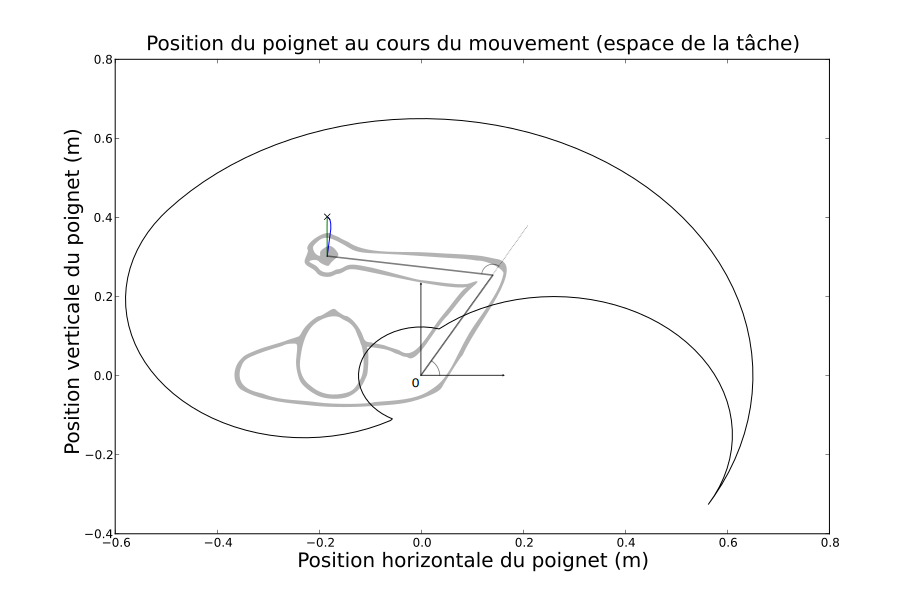
\includegraphics[width=.95\linewidth]{fig/cost_2}
            \end{center}
        \end{column}
        \begin{column}{0.40\textwidth}
            \begin{block}{Résultats}
                \begin{itemize}
                    \item Coût~: +40\%
                    \item Temps de calcul divisé par 3
                \end{itemize}
            \end{block}
        \end{column}
    \end{columns}
\end{frame}

%\begin{frame}{Relation amplitude/durée du mouvement}
%    \begin{itemize}
%        \item Propriété observée par $[$Gordon et al. 94$]$
%        \item Relation linéaire entre la durée du mouvement et son amplitude
%    \end{itemize}
%    \begin{figure}
%        \centering
%        \subfigure{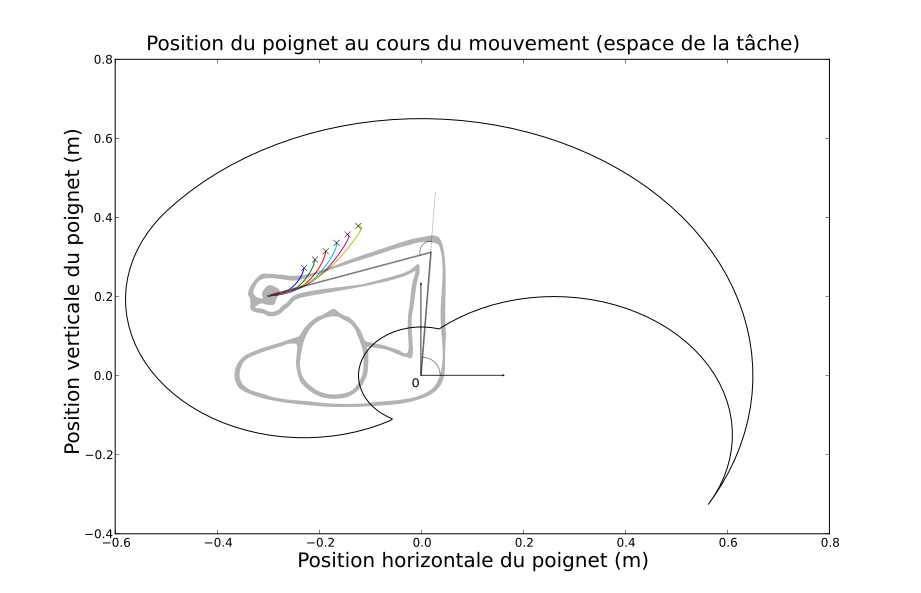
\includegraphics[width=.40\linewidth]{fig/lqp_scaling_paths_2}}~~~
%        \subfigure{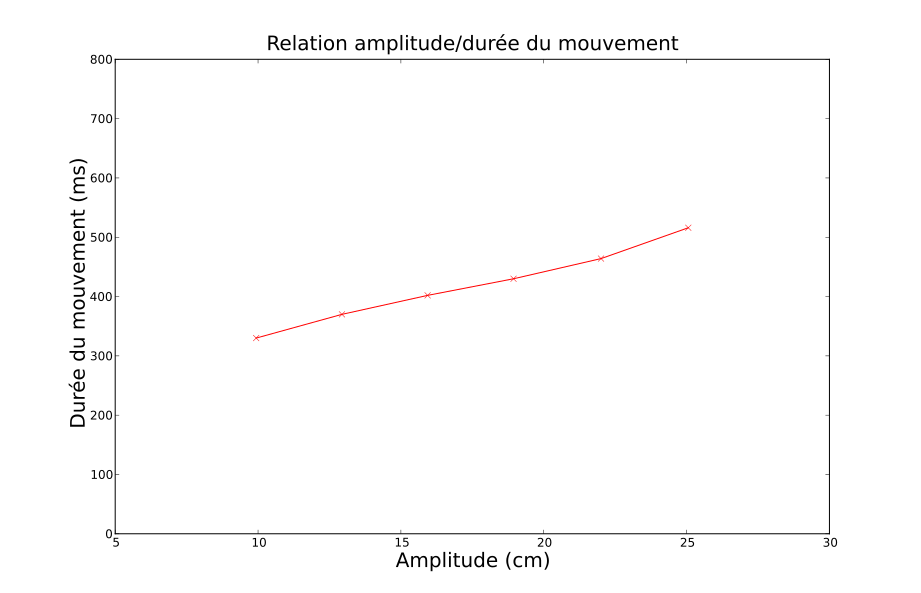
\includegraphics[width=.40\linewidth]{fig/lqp_scaling}}
%    \end{figure}
%    \begin{block}{Résultats}
%        $\qopslqp$ reproduit cette propriété
%    \end{block}
%\end{frame}
%
%\begin{frame}{Anisotropie}
%    \begin{itemize}
%        \item Propriété observée par $[$Gordon et al. 94$]$
%        \item Relation entre la durée du mouvement et sa direction
%    \end{itemize}
%    \begin{figure}
%        \centering
%        \subfigure{\includegraphics[width=.40\linewidth]{fig/lqp_anisotropie_paths_2}}~~~
%        \subfigure{\includegraphics[width=.40\linewidth]{fig/lqp_anisotropy_2}}
%    \end{figure}
%    \begin{block}{Résultats}
%        $\qopslqp$ reproduit cette propriété
%    \end{block}
%\end{frame}

\begin{frame}{Loi de Fitts}
    \begin{small}
        \begin{itemize}
            \item Propriété observée par $[$Fitts 54$]$
            \item Relation entre la durée du mouvement et son indice de difficulté
        \end{itemize}
    \end{small}
    \begin{center}
        \includegraphics[width=.55\linewidth]{fig/fitts_exp2}
    \end{center}
\end{frame}

\begin{frame}{Loi de Fitts}
    \begin{figure}
        \centering
        \subfigure{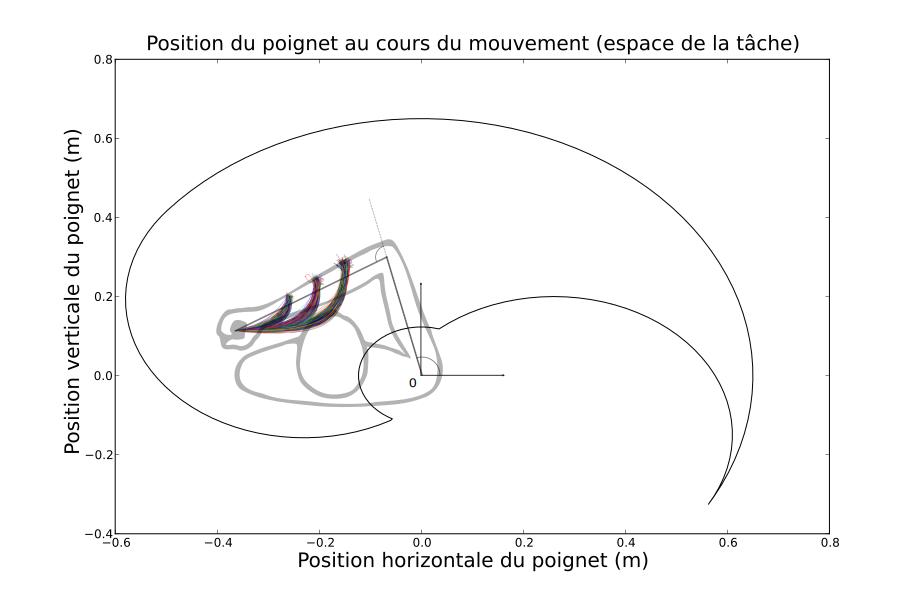
\includegraphics[width=.40\linewidth]{fig/lqp_fitts_paths_light2}}~~~
        \subfigure{\includegraphics[width=.40\linewidth]{fig/lqp_fitts2_sigma4_2}}
    \end{figure}
    \begin{block}{Résultats}
        $\qopslqp$ reproduit cette propriété
    \end{block}
\end{frame}

\begin{frame}{Profil de variabilité}
    \begin{small}
        \begin{itemize}
            \item Propriété observée par $[$Selen et al. 06$]$
            \item Variabilité maximale en milieu de mouvement, minimale à la fin
        \end{itemize}
    \end{small}
    \begin{center}
        \includegraphics[width=.70\linewidth]{fig/lqp_variations_paths4}
    \end{center}
\end{frame}

\begin{frame}{Profil de variabilité}
    \begin{figure}
        \centering
        \subfigure[$\qopslqp$]{\includegraphics[width=.40\linewidth]{fig/variabilite}}~~~
        \subfigure[Selen et al. 06]{\includegraphics[width=.40\linewidth]{fig/selen06}}
    \end{figure}
    \begin{block}{Résultats}
        $\qopslqp$ reproduit cette propriété
    \end{block}
\end{frame}



\section{Limites et perspectives}

\subsection{}

\begin{frame}{Les limites de l'étude}
    Modèle mécanique simple
    \begin{itemize}
        \item Bras 2D
        \item Seulement 2 articulations
        \item Pas de redondance du bras dans l'espace de la tâche ($\ostate \rightarrow \jstate$)
    \end{itemize}
    ~\\
    Modèle de muscle simplifié
    \begin{itemize}
        \item Modèle linéaire
        \item Pas d'élasticité
        \item Modèle réactif
    \end{itemize}
    ~\\
    Coût énergétique des solutions trop élevé
\end{frame}

\begin{frame}{Perspectives}
    \begin{columns}
        \begin{column}{0.50\textwidth}
            Apprentissage du contrôle moteur
            \begin{itemize}
                \item Apprendre dans l'espace de la tâche
                \item Vaincre la \og{}malédiction de la dimensionalité\fg{}
                \item L'adaptation motrice et la réoptimisation
            \end{itemize}
        \end{column}
        \begin{column}{0.50\textwidth}
            \begin{center}
                \includegraphics[width=.95\linewidth]{fig/icub3_light}
            \end{center}
        \end{column}
    \end{columns}
\end{frame}


\appendix

\section{Annexes}

\begin{frame}{Dynamique du bras dans l'espace de la tâche}
    \begin{small}
        \begin{align}
            \x   & = \fk(\q) \\
            \dx  & = \jacobian(\q)\dq \\
            \vt  & = \ms{M}(\q) ~ \ddq + \vs{n}(\q, \dq) \\
            \ddq & = \ms{M}^{-1}(\q) ~ \vt - \ms{M}^{-1}( \q ) ~ \vs{n}( \q, \dq ) \\
            \ddx & = \jacobian(\q) \ddq + \djacobian(\q, \dq) \dq \\
            \ddx & = \jacobian(\q) ~ \ms{M}^{-1}(\q) ~ \vt - \jacobian(\q) ~ \ms{M}^{-1}(\q) ~ \vs{n}( \q, \dq ) + \djacobian(\q, \dq) ~ \dq \\
            \vt  & = \jacobian^T(\q) ~ \octrl \\
            \ddx & = \jacobian(\q) ~ \ms{M}^{-1}(\q) ~ \jacobian^T(\q) ~ \octrl - \jacobian(\q) ~ \ms{M}^{-1}(\q) ~ \vs{n}( \q, \dq ) + \djacobian(\q, \dq) ~ \dq
        \end{align}
    \end{small}
\end{frame}



\end{document}
